\documentclass[12pt, compress, xcolor=table]{beamer}
\usetheme[titleprogressbar]{metropolis}

\usepackage{booktabs}
\usepackage[scale=2]{ccicons}

\usepackage{caption}
\captionsetup[figure]{font=scriptsize,labelfont=scriptsize}
\setlength{\belowcaptionskip}{-10pt}

\title{Localization of a Sounding Rocket via GPS}
\author{Simon Herzog}
\institute{Final Presentation Bachelor Thesis}
\date{June, 2018}

\begin{document}


\maketitle

\begin{frame}{Table of Contents}
 \tableofcontents
\end{frame}


\section{Assignment}

\begin{frame}{Assignment}
 \begin{itemize}
  \setlength\itemsep{0.5cm}
  \item Evaluate GPS positioning for a sounding rocket
  \item Determine external and internal error sources
  \item Find error mitigation methods
  \item Demonstrate feasibility of one method
 \end{itemize}
\end{frame}

\begin{frame}{Requirements}
 \begin{itemize}
  \setlength\itemsep{0.5cm}
  \item Vertical RMS error $\le$ 1 meter
  \item GPS fix max. 2 seconds after burnout
  \item Uplink data rate max. 2 kbit/s
 \end{itemize}
\end{frame}


\section{GPS Concept for a Sounding Rocket}

\begin{frame}{Special Conditions}
 \begin{columns}
 
  \column{0.7\textwidth}
  \begin{itemize}
   \setlength\itemsep{0.5cm}
   \item 10 g acceleration
   \item Signal fading due to rotation
   \item Telemetry transmitter interference
  \end{itemize}
  
  \column{0.3\textwidth}
  \begin{figure}
   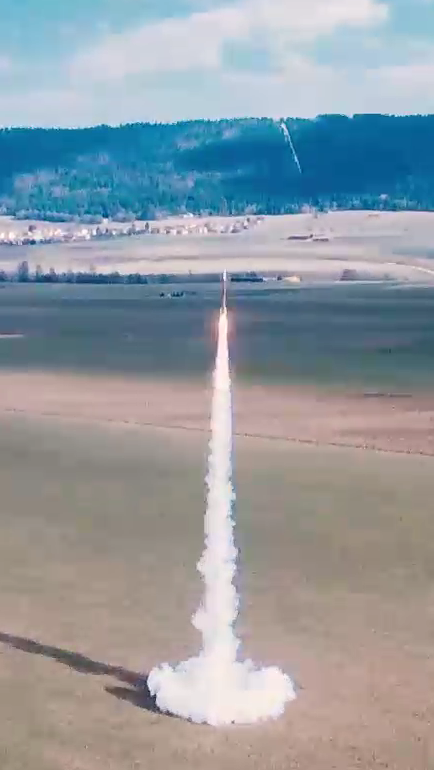
\includegraphics[width=\textwidth]{images/Mestral_Launch.png}
  \end{figure}
 
 \end{columns}
\end{frame}

\begin{frame}{Accuracy Enhancement Method Selection}
 \begin{columns}
  
  \column{0.5\textwidth}
  \begin{itemize}
   \setlength\itemsep{0.5cm}
   \item Dual Frequency Measurements
   \item Carrier-Phase Measurements
   \item Differential GPS
  \end{itemize}
  
  \column{0.5\textwidth}
  \begin{figure}
   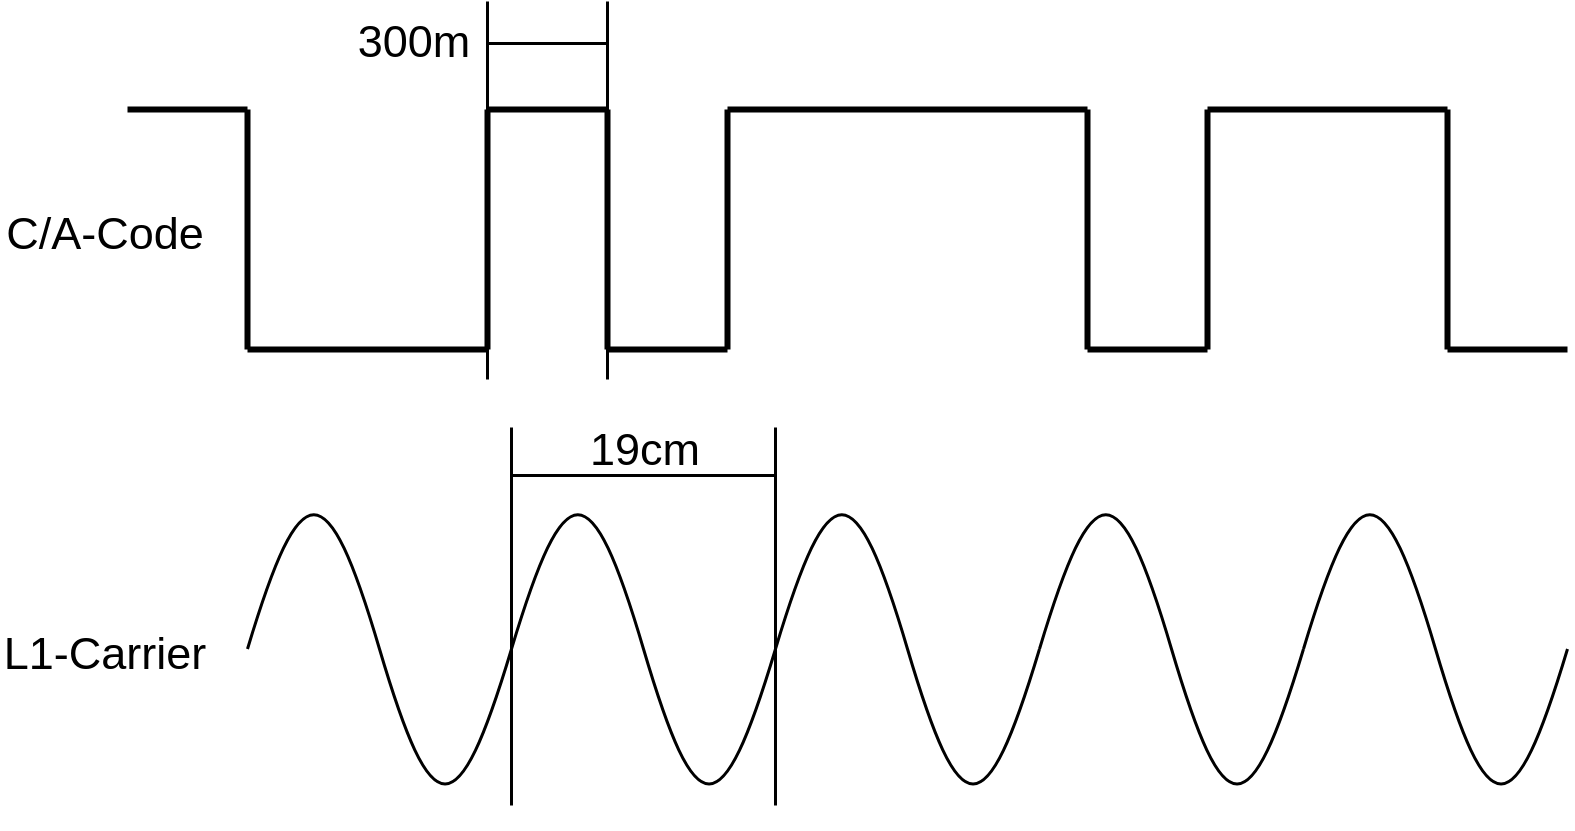
\includegraphics[width=\textwidth]{images/Carrier_Phase_Measurement.png}
   
   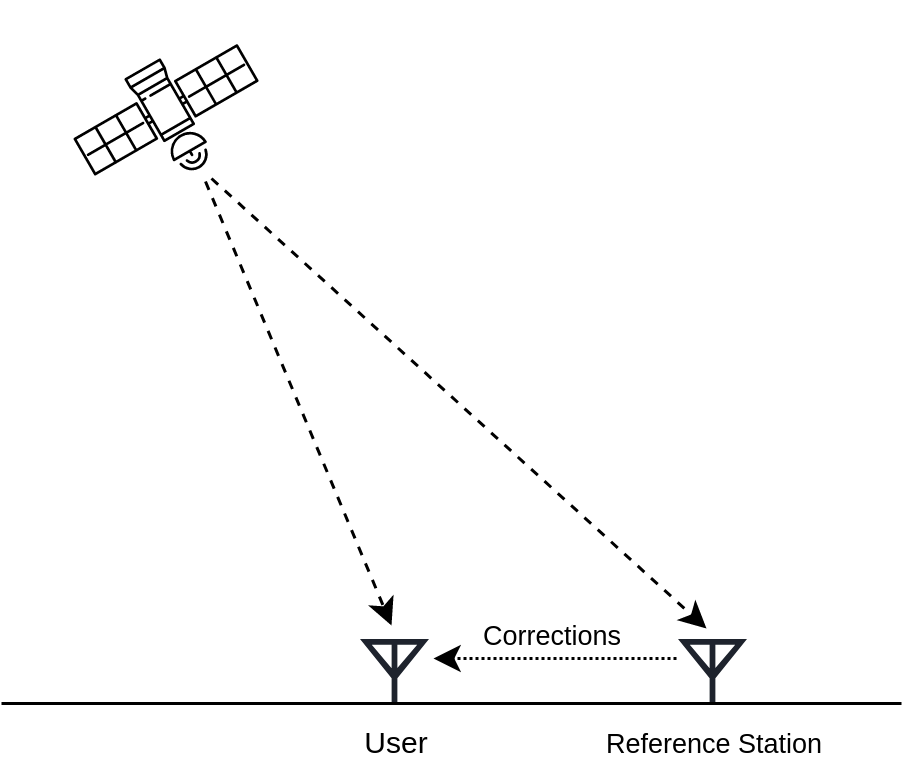
\includegraphics[height=4cm]{images/Differential_GPS.png}
  \end{figure}
  
 \end{columns}
\end{frame}

\begin{frame}{DGPS Concept}
 \begin{columns}
  
  \column{0.6\textwidth}
  \begin{itemize}
   \setlength\itemsep{0.5cm}
   \item Self-generated pseudorange corrections
   \item Reference station at ground station
   \item Correction transmission over RF telemetry link
   \item Applycation of corrections by COTS GPS receiver
  \end{itemize}
  
  \column{0.4\textwidth}
  \begin{figure}
   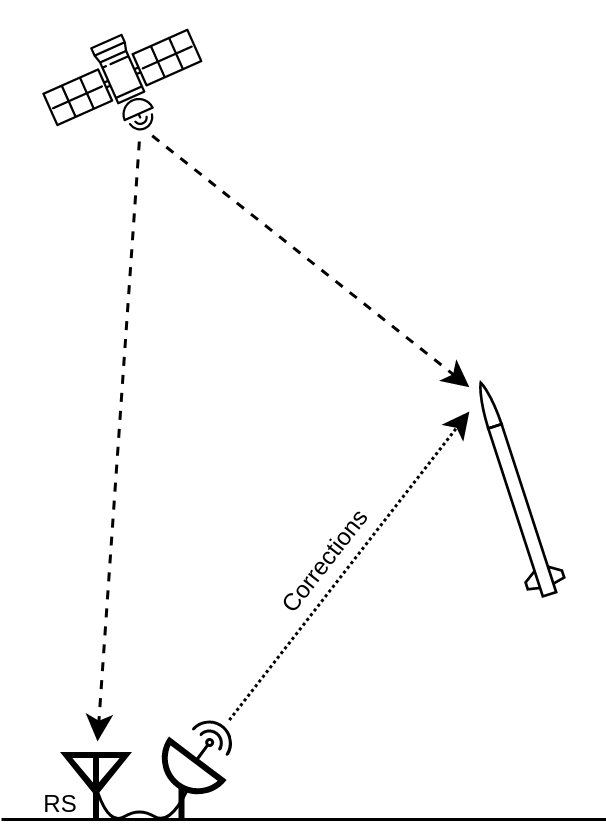
\includegraphics[width=\textwidth]{images/DGPS_Rocket_Concept.png}
  \end{figure}
  
 \end{columns}
\end{frame}


\section{TELL Framework}

\begin{frame}{TELL Rocket}
 \begin{figure}
  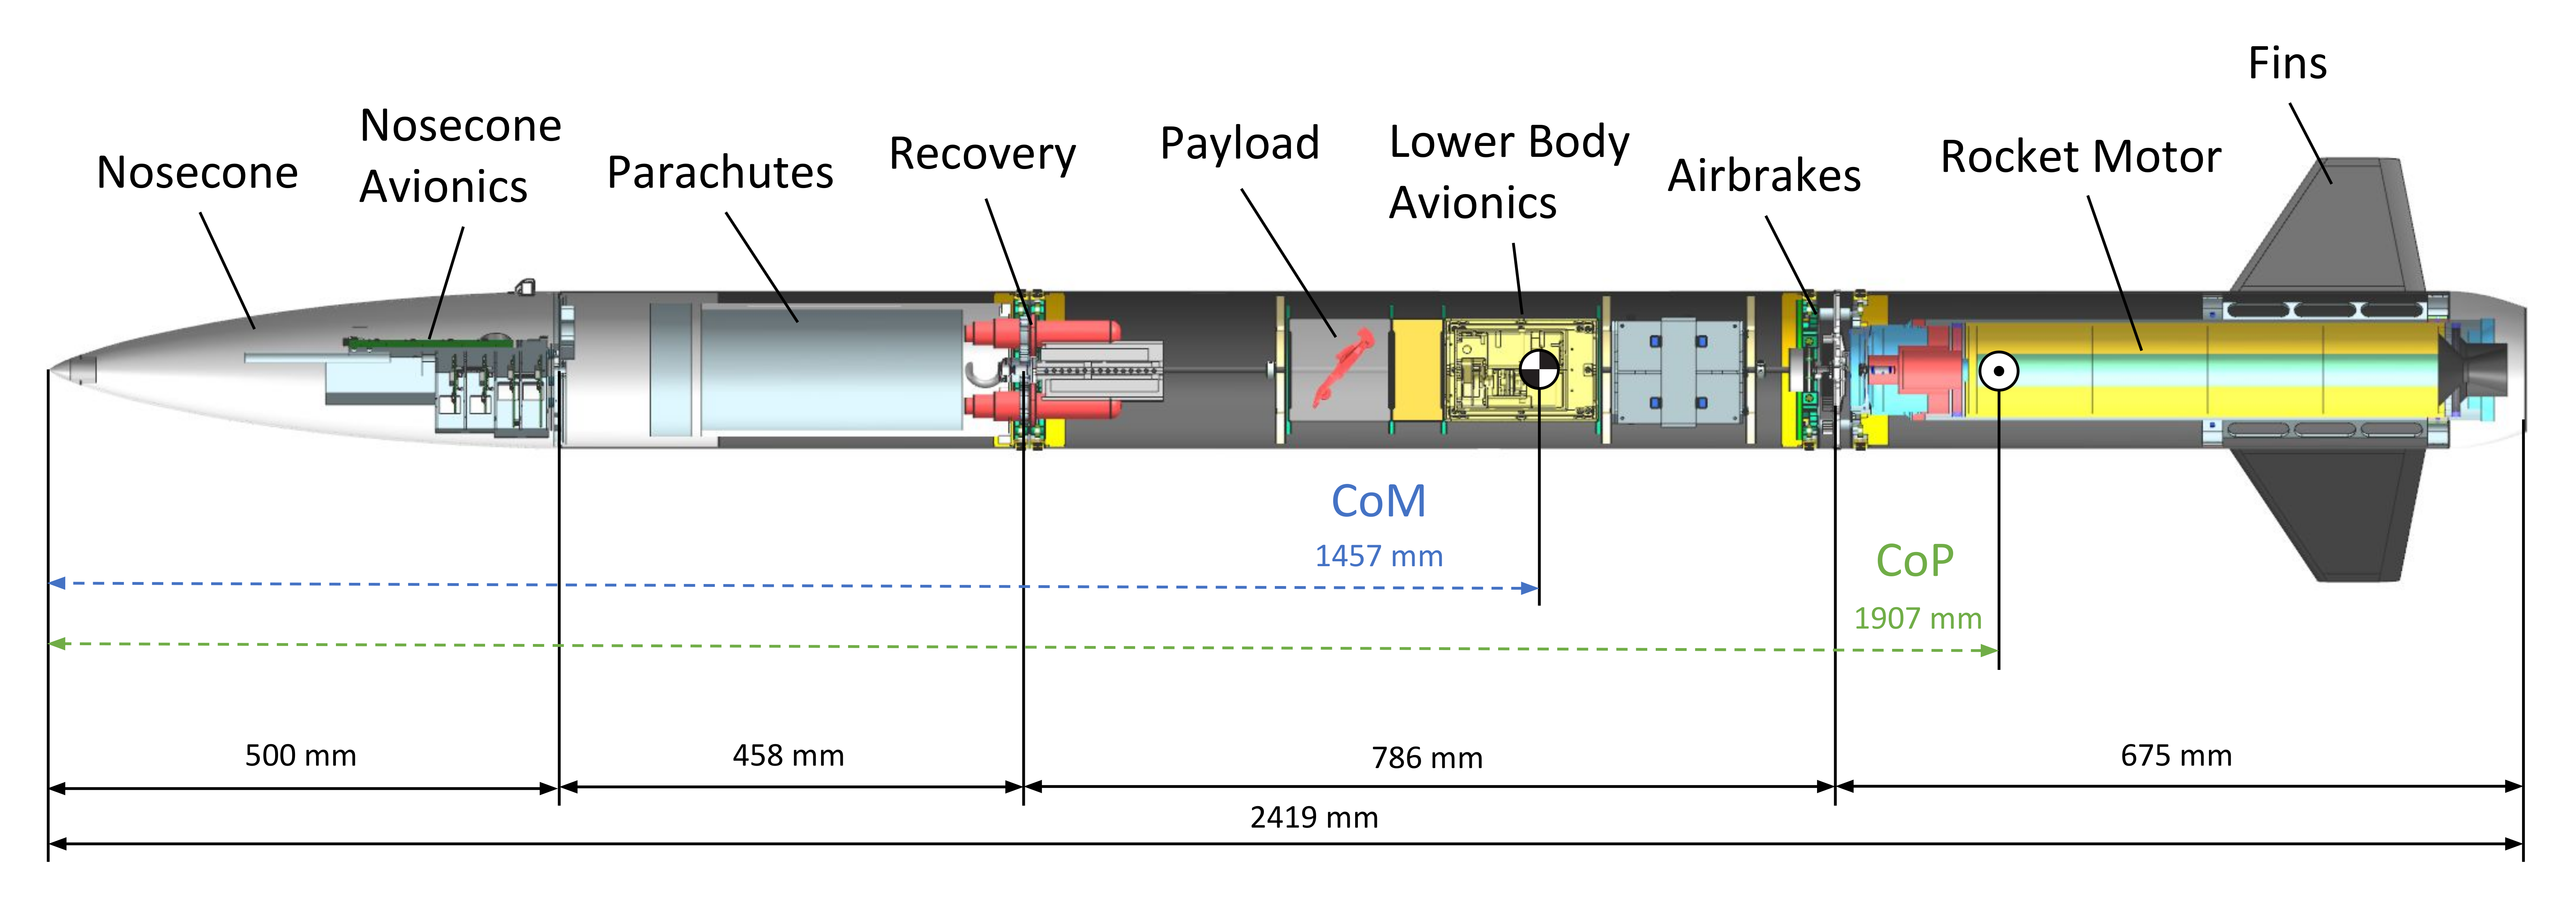
\includegraphics[width=\textwidth]{images/TELL_Structure.png}
 \end{figure}
\end{frame}

\begin{frame}{TELL Avionics}
 \begin{columns}
  
  \column{0.6\textwidth}
  \begin{itemize}
   \setlength\itemsep{0.5cm}
   \item Nose cone and lower body avionics
   \item Sensor data logging
   \item Telemetry downlink
   \item 2 GPS receivers
   \item Air brake control
  \end{itemize}
  
  \column{0.4\textwidth}
  \begin{figure}
   \centering
   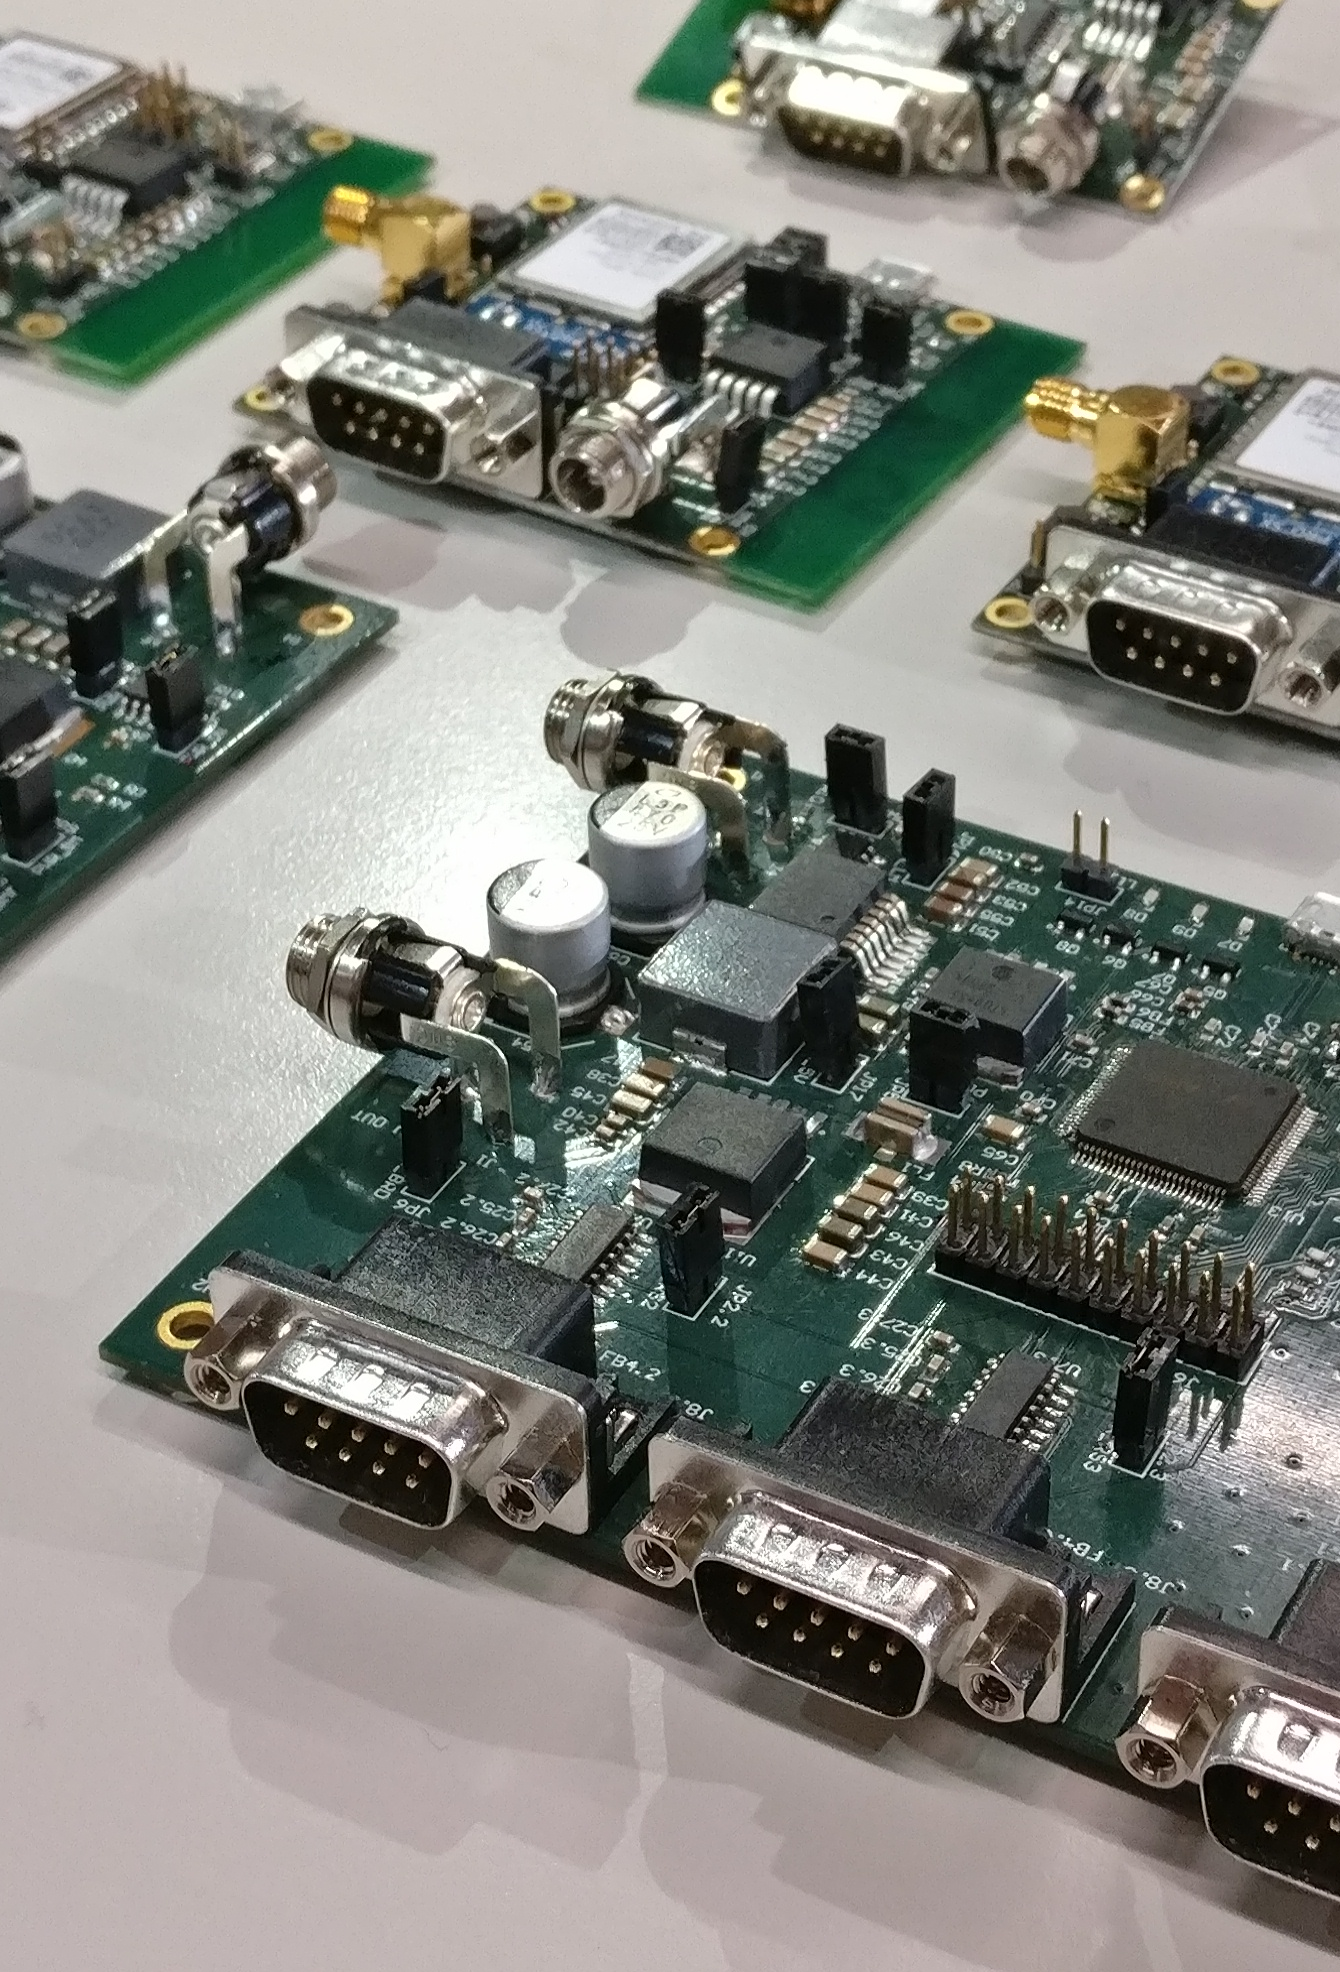
\includegraphics[width=\textwidth]{images/Avionics.png}
  \end{figure}
  
 \end{columns}
\end{frame}

\begin{frame}{TELL Ground Station}
 \begin{itemize}
  \setlength\itemsep{0.5cm}
  \item Laptop as the central device
  \item Telemetry receiver with directional antenna
  \item GPS receiver for post-prcessing DGPS reference station
 \end{itemize}
\end{frame}


\section{Implementation}

\begin{frame}{Top Level Data Flow}
 \begin{figure}
  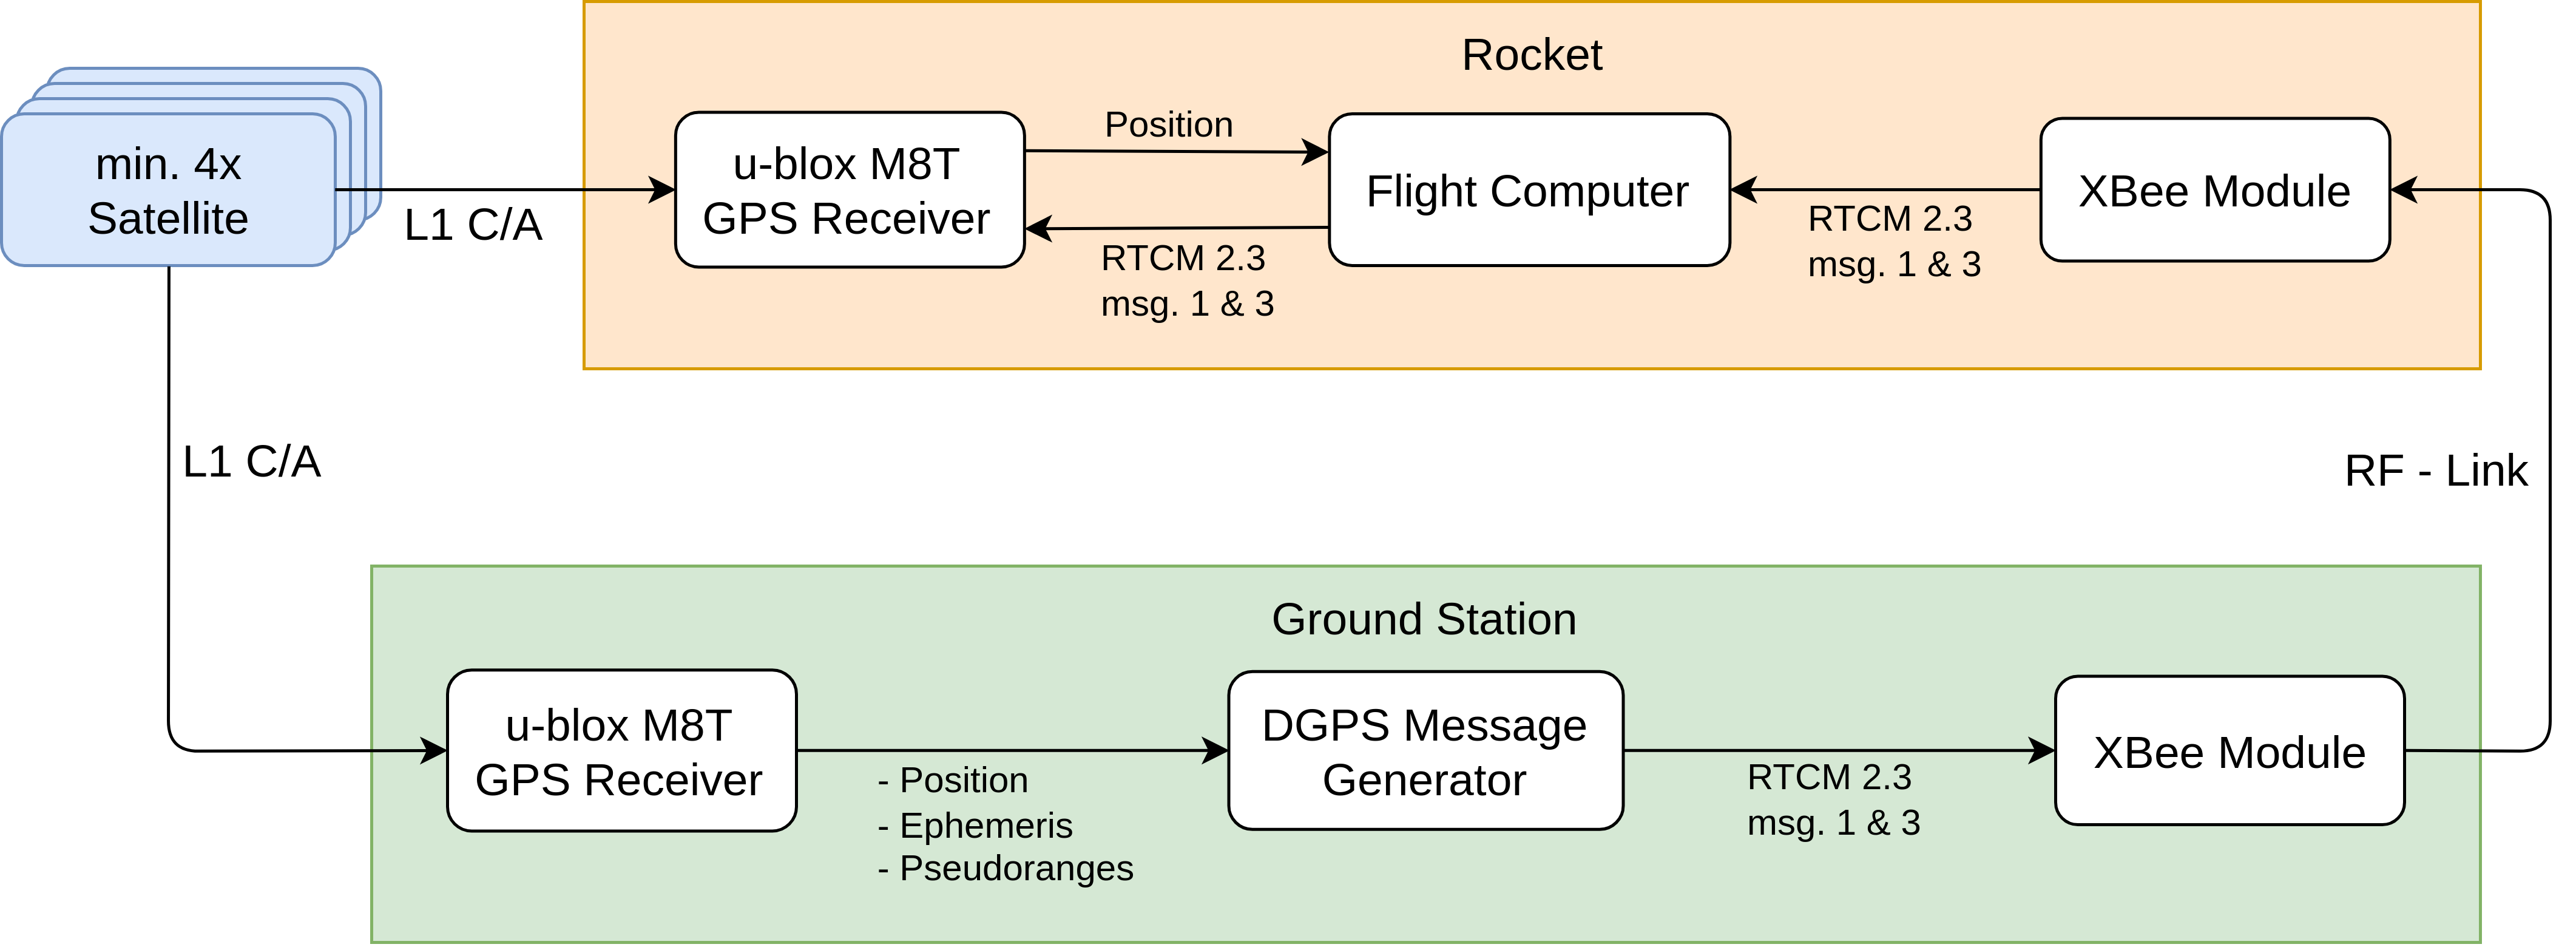
\includegraphics[width=\textwidth]{images/DGPS_System_Overview.png}
 \end{figure}
\end{frame}

\begin{frame}{GPS Receiver}
 \begin{columns}
  
  \column{0.6\textwidth}
  \begin{itemize}
   \setlength\itemsep{0.5cm}
   \item u-blox M8T receiver
   \item outputs GPS raw data
   \item can receive and apply RTCM 2.3 messages
  \end{itemize}
  
  \column{0.4\textwidth}
  \begin{figure}
   \centering
   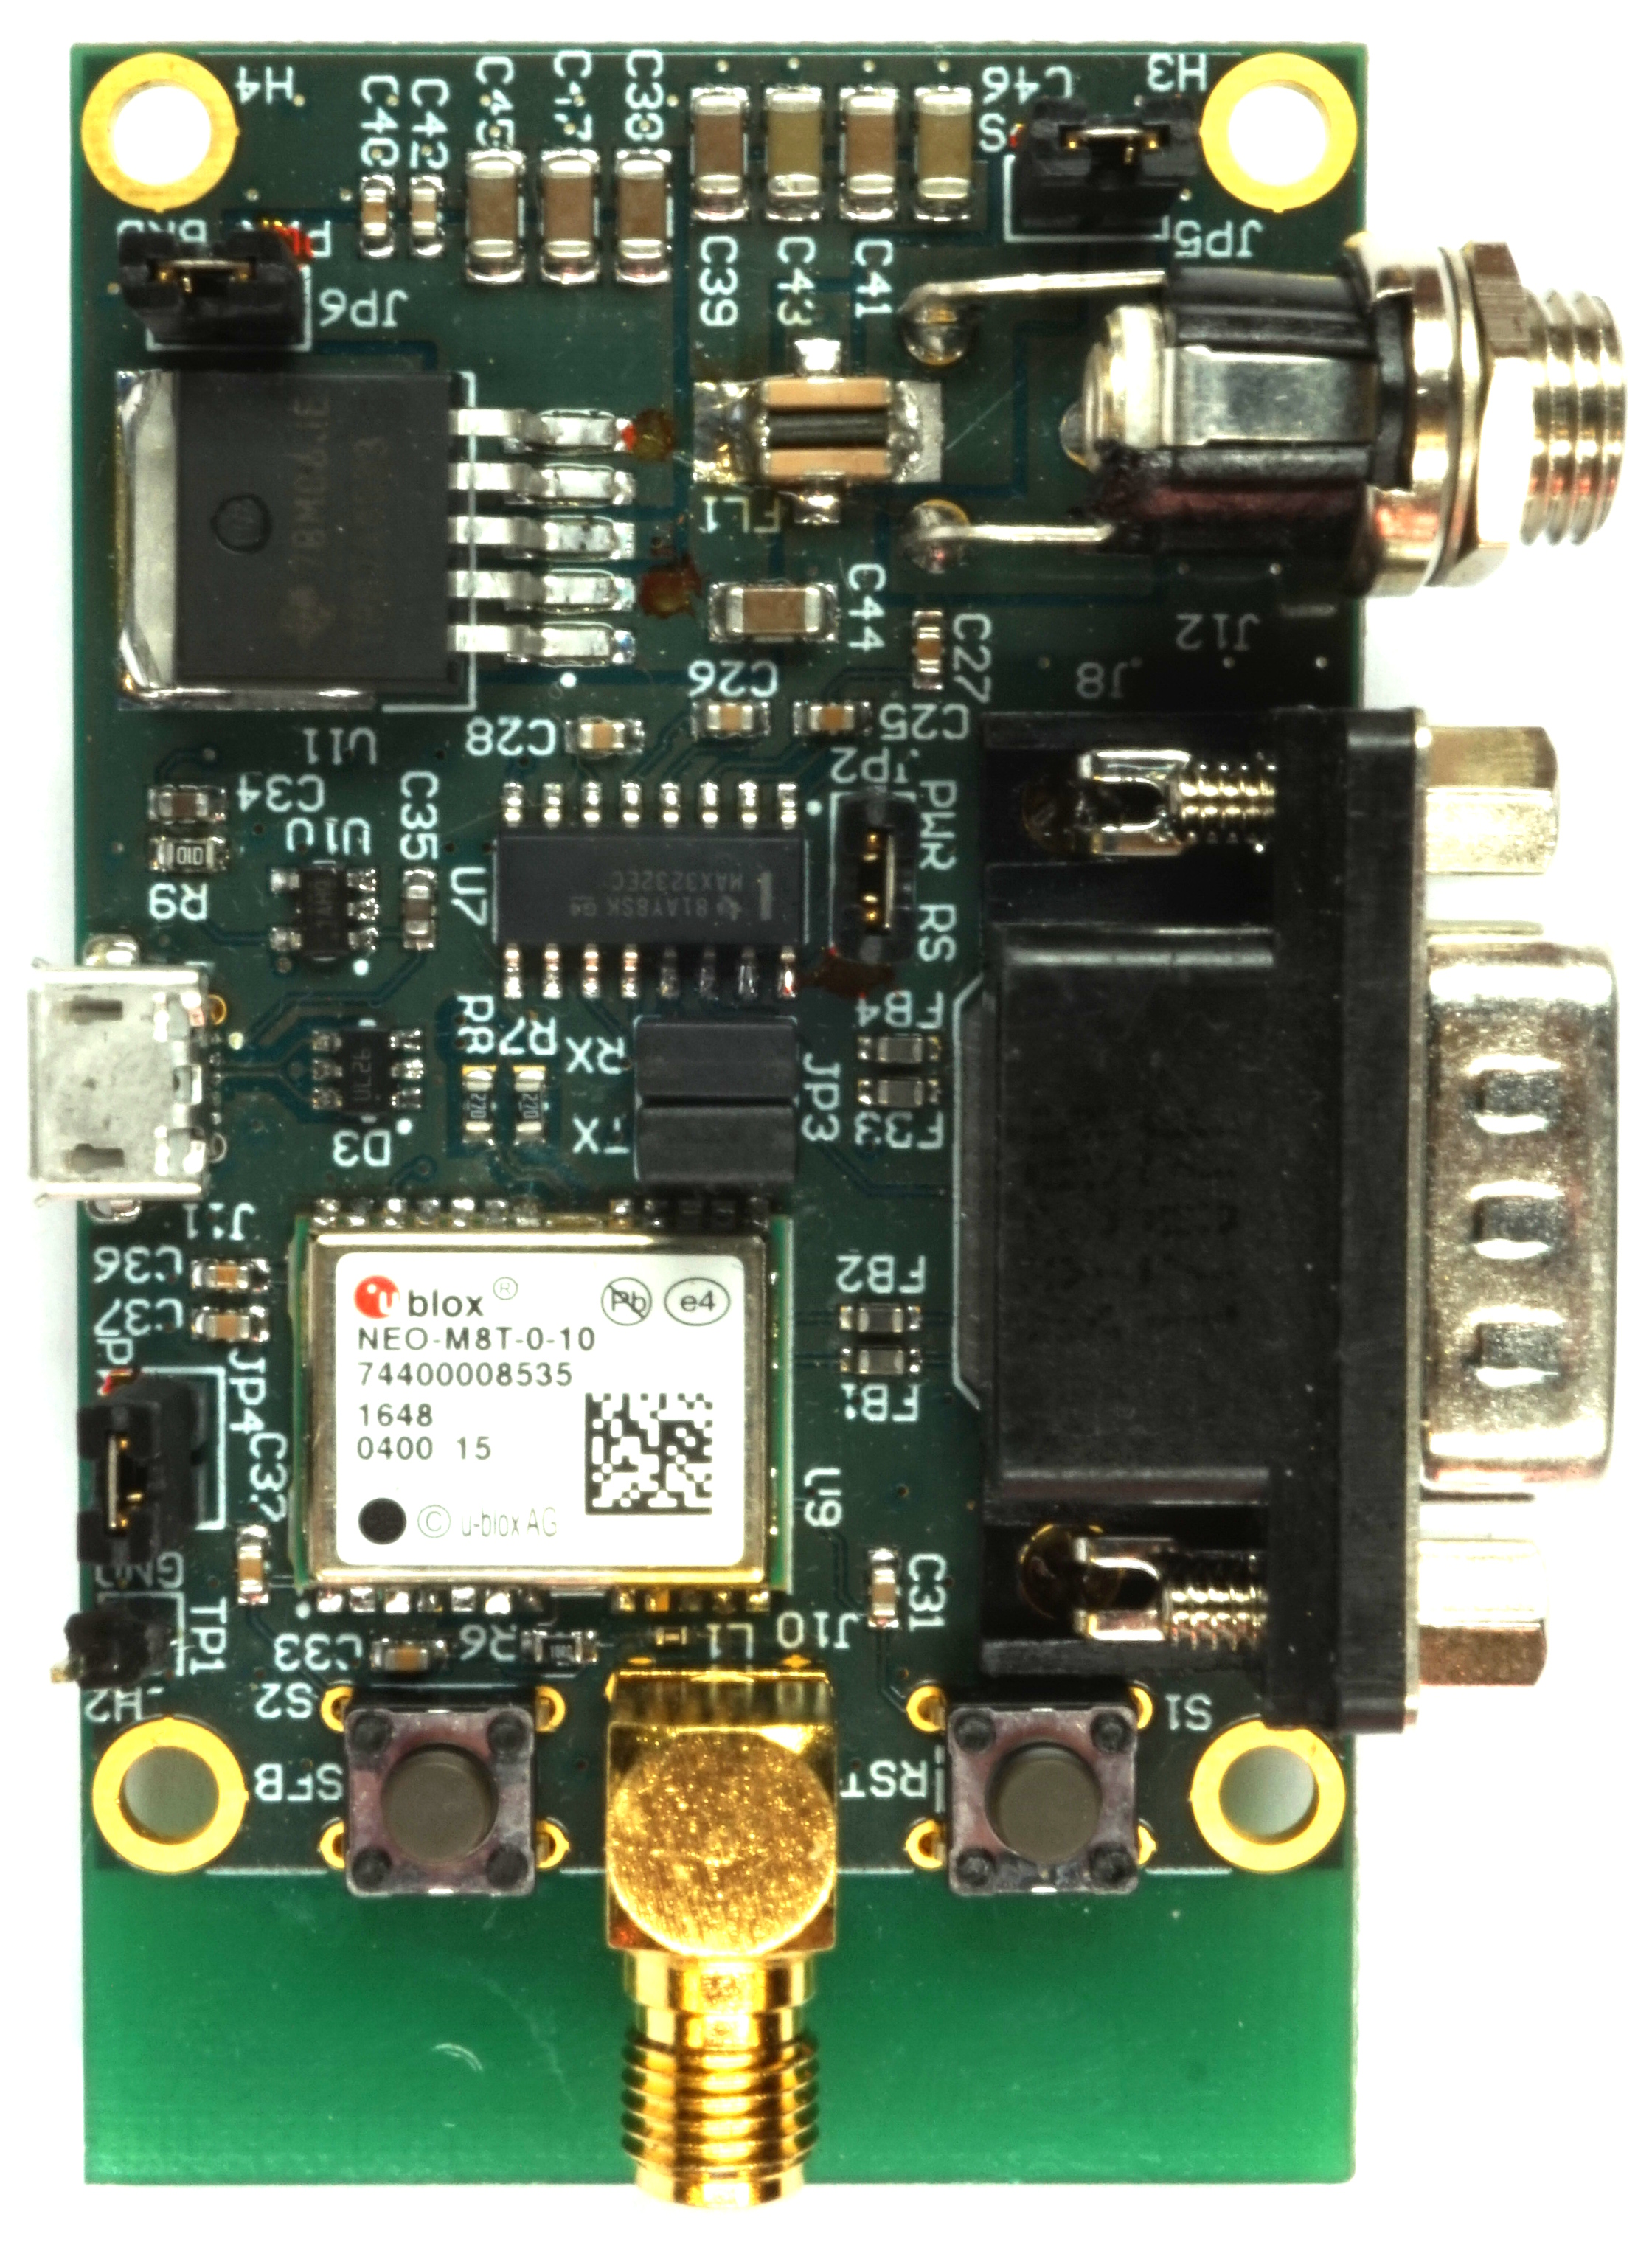
\includegraphics[width=\textwidth]{images/M8T_Receiver_Board.jpg}
  \end{figure}
  
 \end{columns}
\end{frame}

\begin{frame}{DGPS Message Generator Software Architecture}
 \begin{figure}
  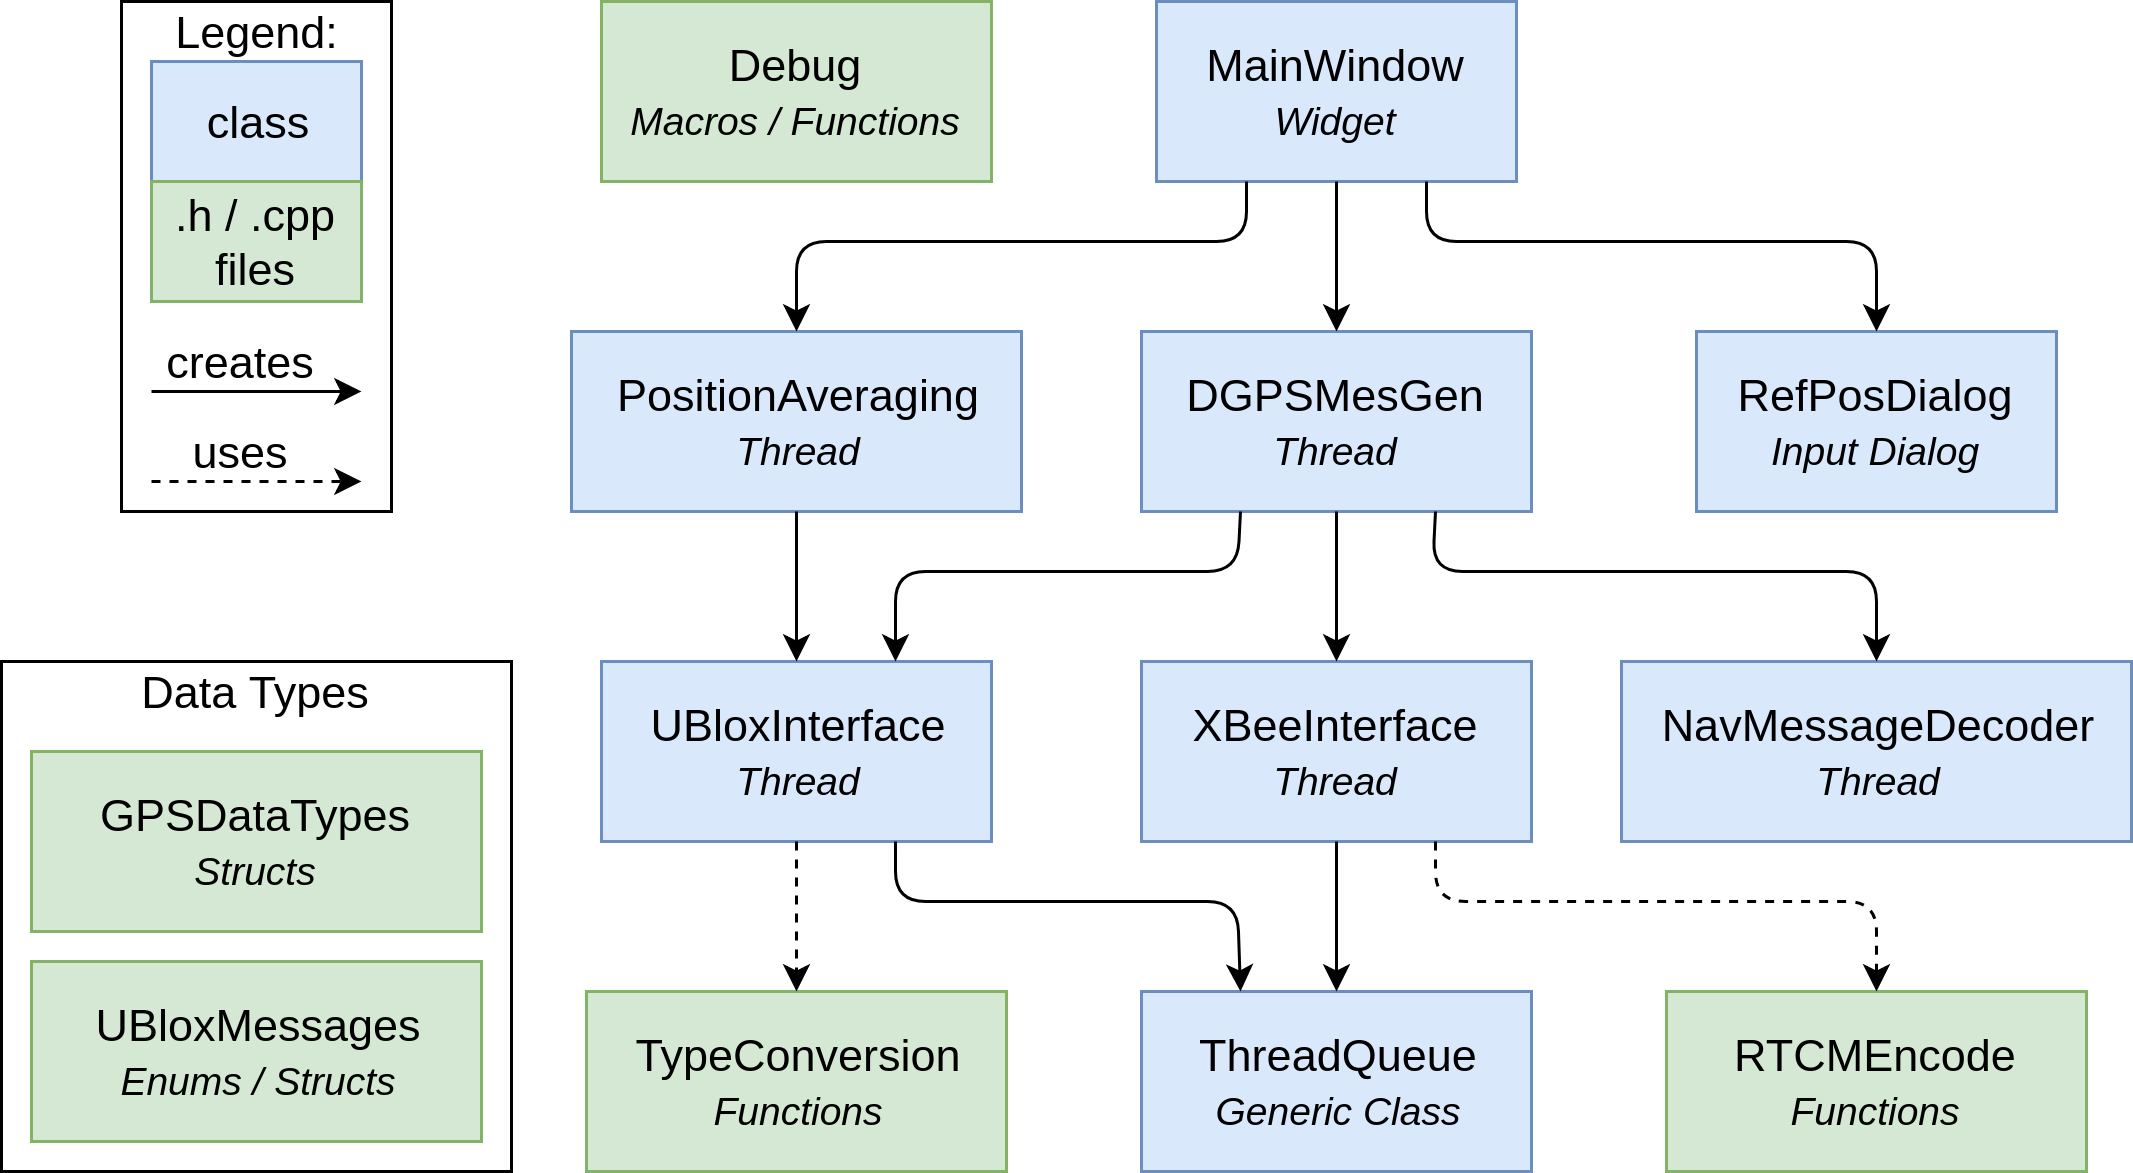
\includegraphics[width=\textwidth]{images/Software_Architecture.png}
 \end{figure}
\end{frame}

\begin{frame}{DGPS Message Generator Data Flow}
 \begin{figure}
  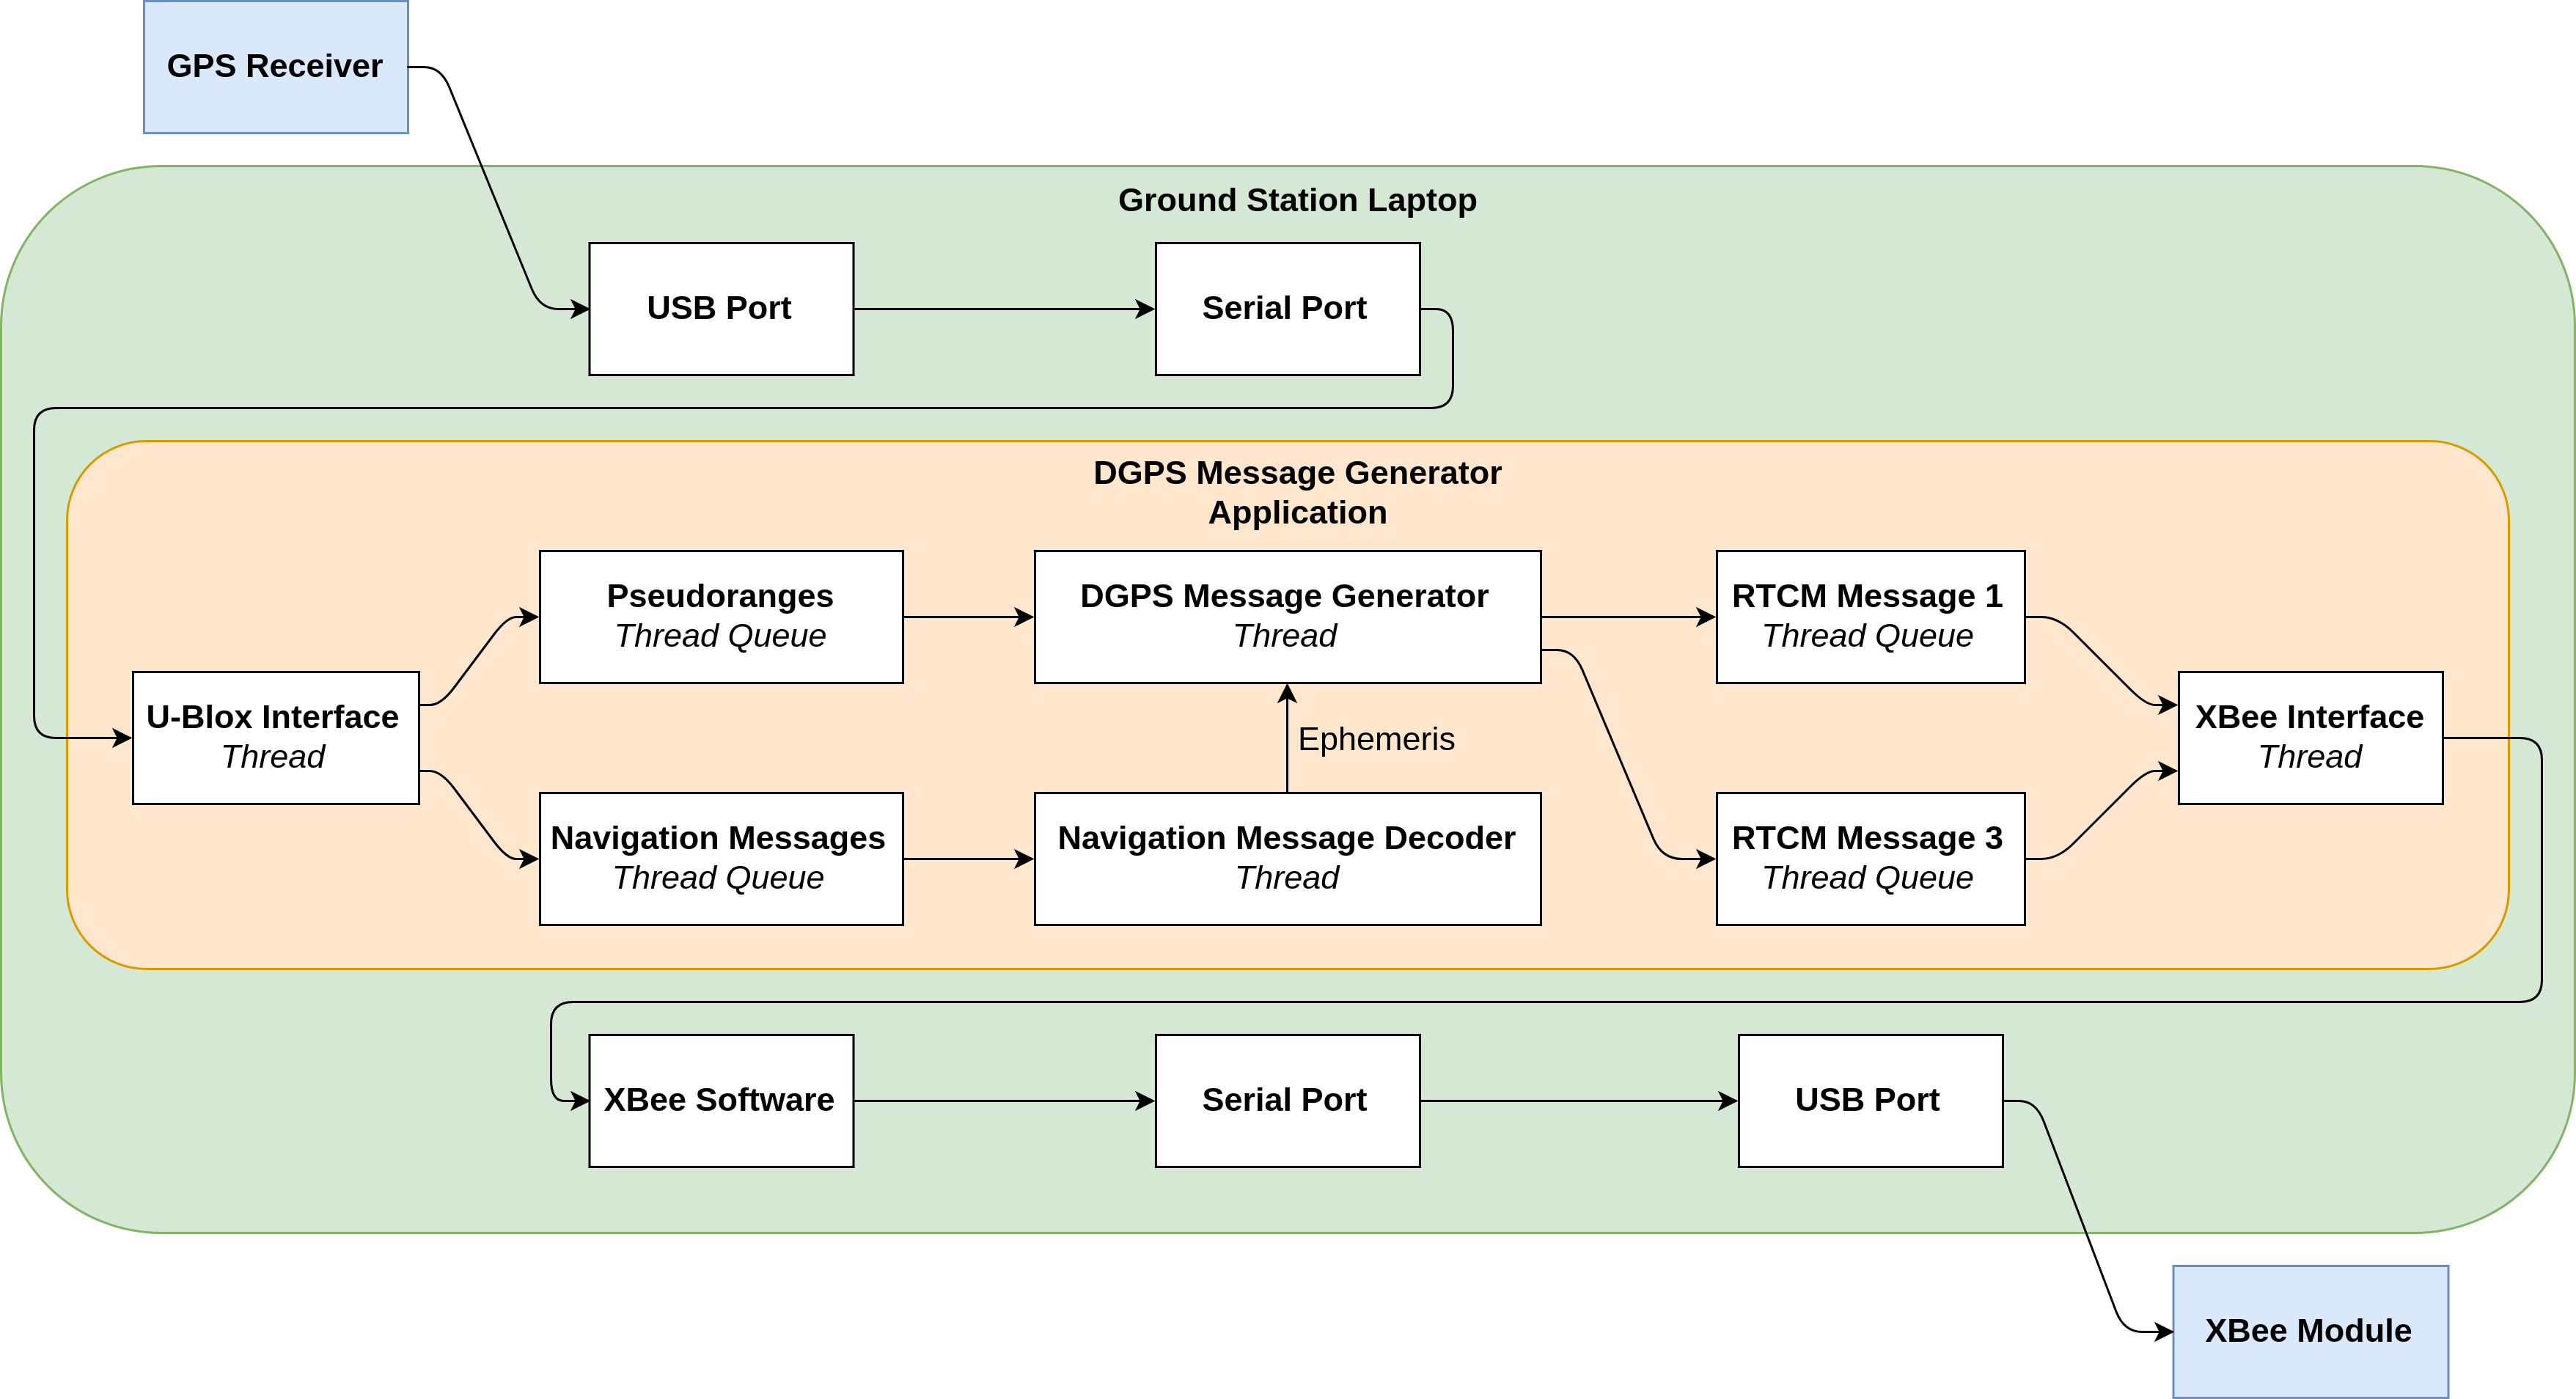
\includegraphics[width=\textwidth]{images/Data_Flow.png}
 \end{figure}
\end{frame}


\section{Testing}

\begin{frame}{Static Test on the Sonnenberg}
 \begin{figure}
  \includegraphics[width=\textwidth]{images/measurement_kriens_setup.png}
 \end{figure}
\end{frame}

\begin{frame}{Receiver Setup}
 \begin{figure}
  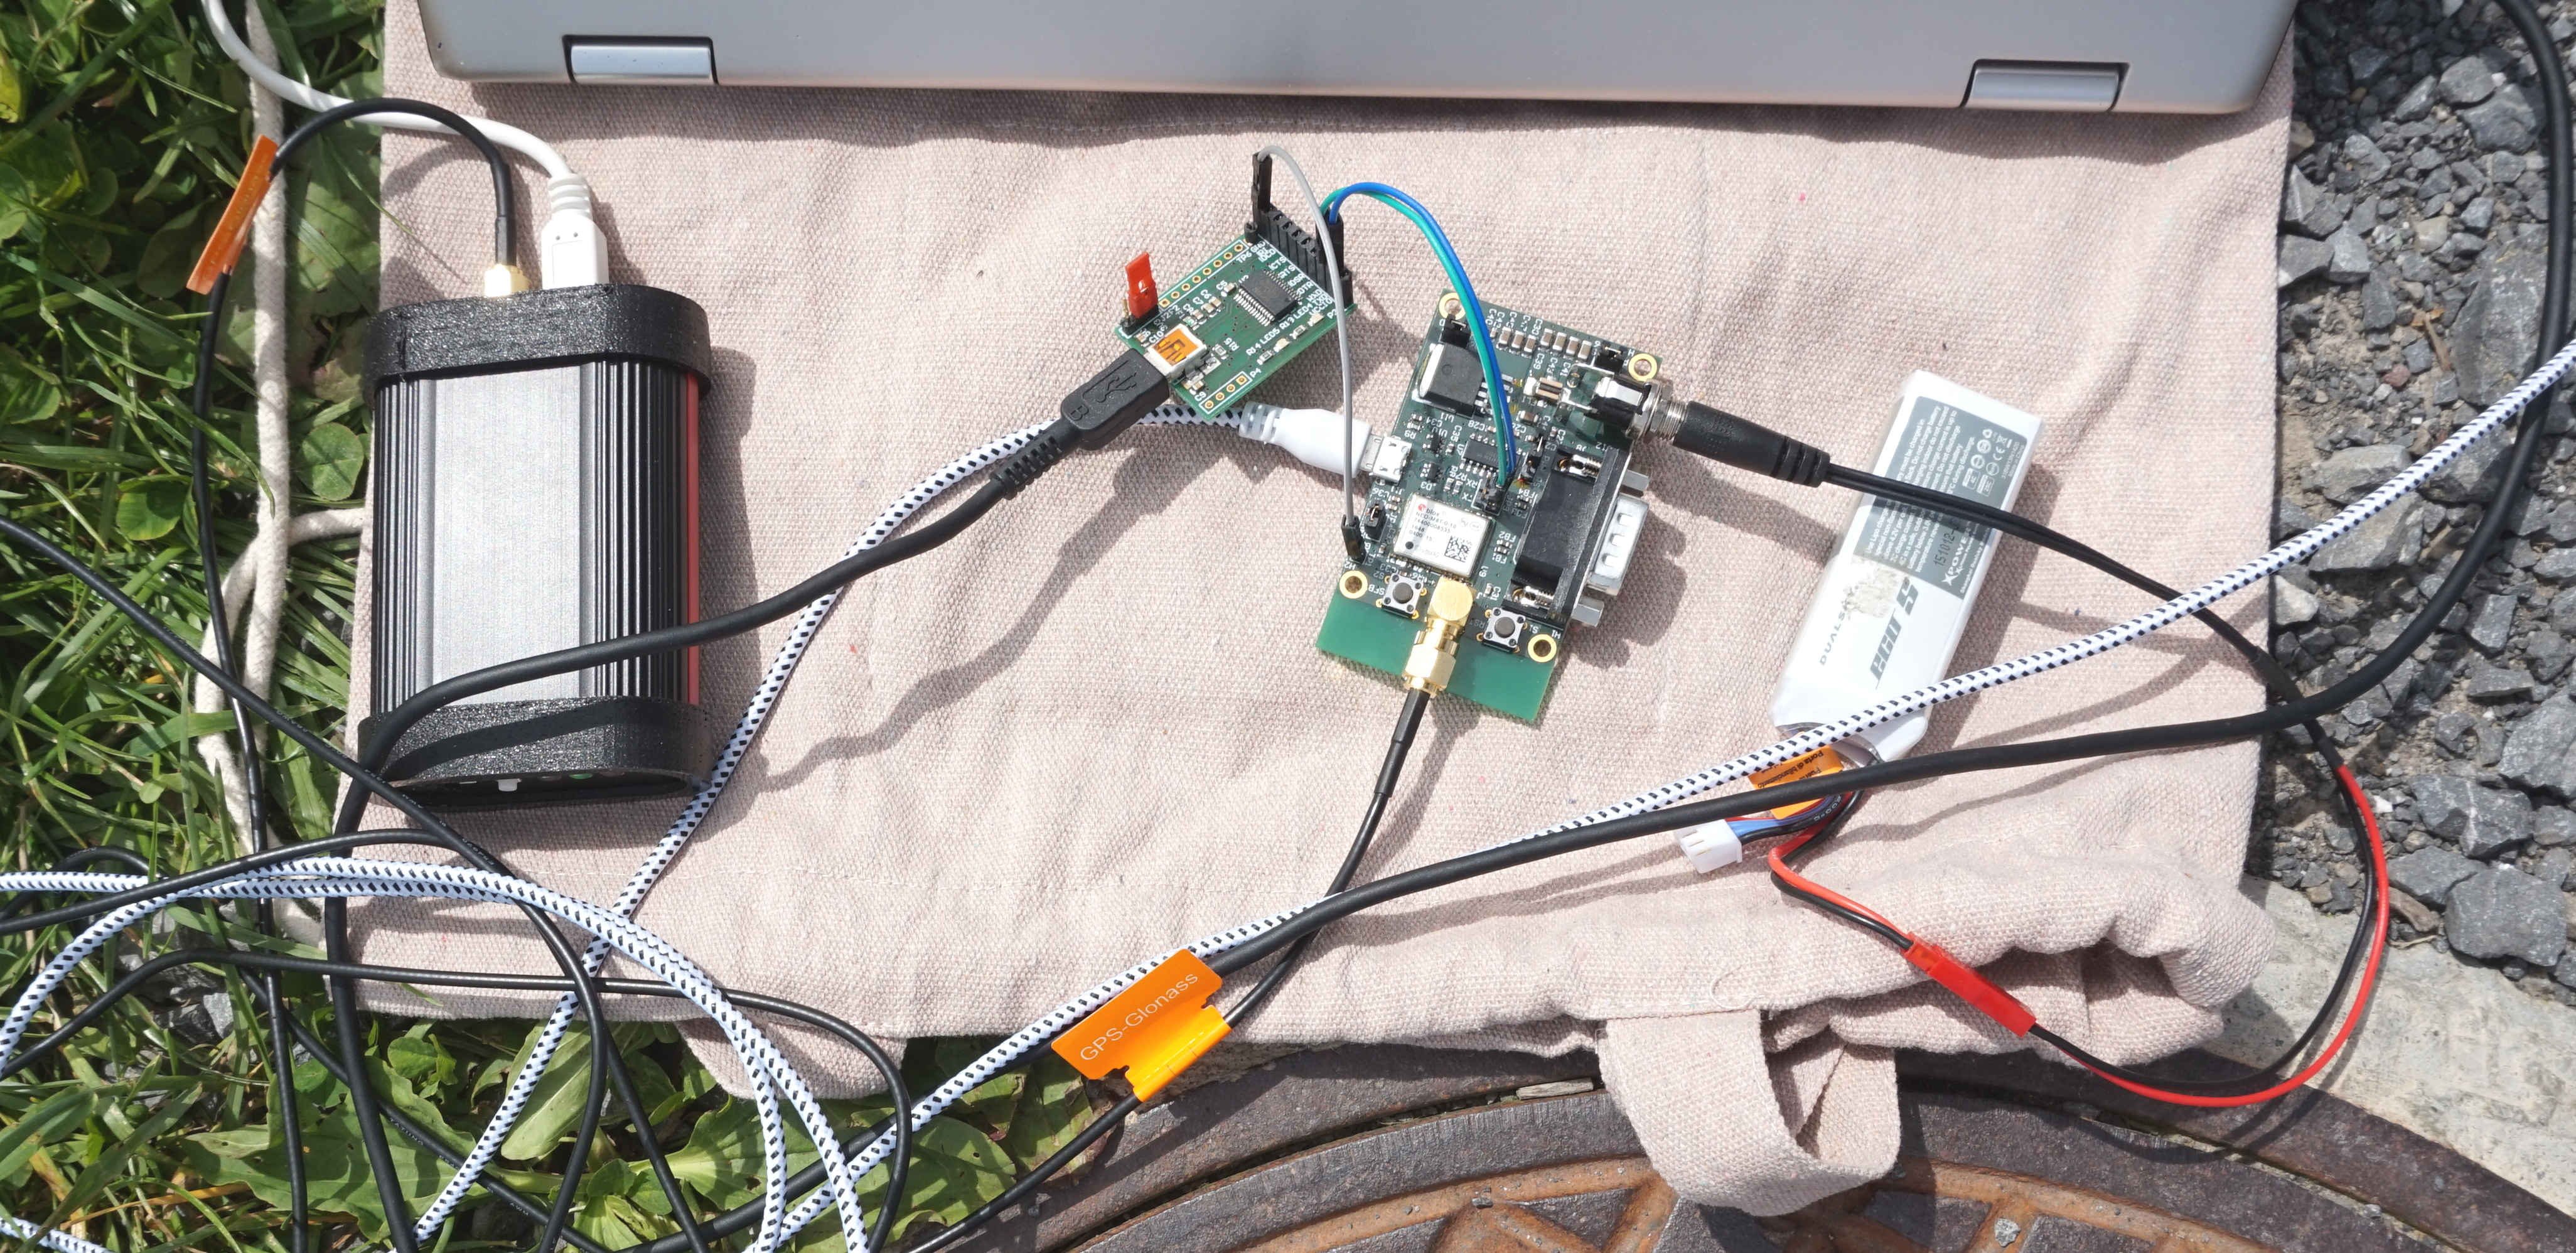
\includegraphics[width=\textwidth]{images/measurement_kriens_receiver.jpg}
 \end{figure}
\end{frame}

\begin{frame}{Sonnenberg: Scatterplot}
 \begin{columns}
  
  \column{0.5\textwidth}
  \begin{table}[]
  \centering
  \scriptsize
  \begin{tabular}{l|ll}
			    & GPS   & DGPS  \\ \hline
  RMS Error 2D {[}m{]}       & 5.816 & 5.647 \\
  RMS Error Vertical {[}m{]} & 1.096 & 4.112 \\
  Bias 2D {[}m{]}            & 4.6   & 4.577 \\
  Bias Vertical {[}m{]}      & 0.215 & 3.456 \\
  1$\sigma$ 2D {[}m{]}       & 3.559 & 3.309 \\
  1$\sigma$ Vertical {[}m{]} & 1.075 & 2.229
  \end{tabular}
  \end{table}
  
  \column{0.5\textwidth}
  \begin{figure}
   \centering
   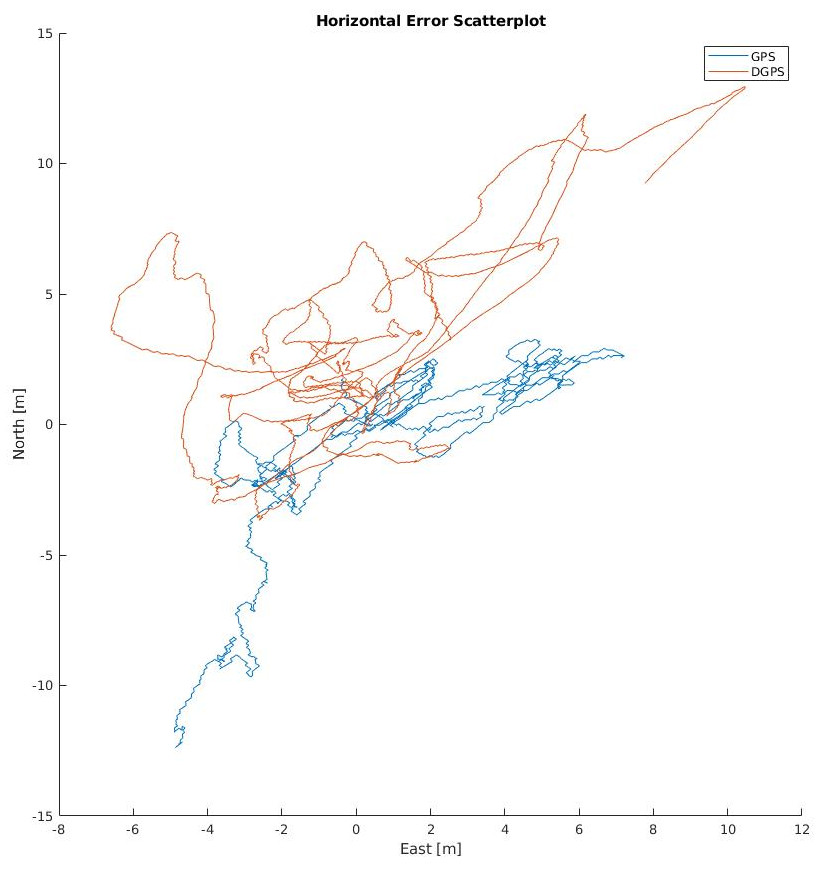
\includegraphics[width=\textwidth]{images/Scatterplot_Kriens.jpg}
  \end{figure}
  
 \end{columns}
\end{frame}

\begin{frame}{Sonnenberg: Position Error}
 \begin{figure}
  \centering
  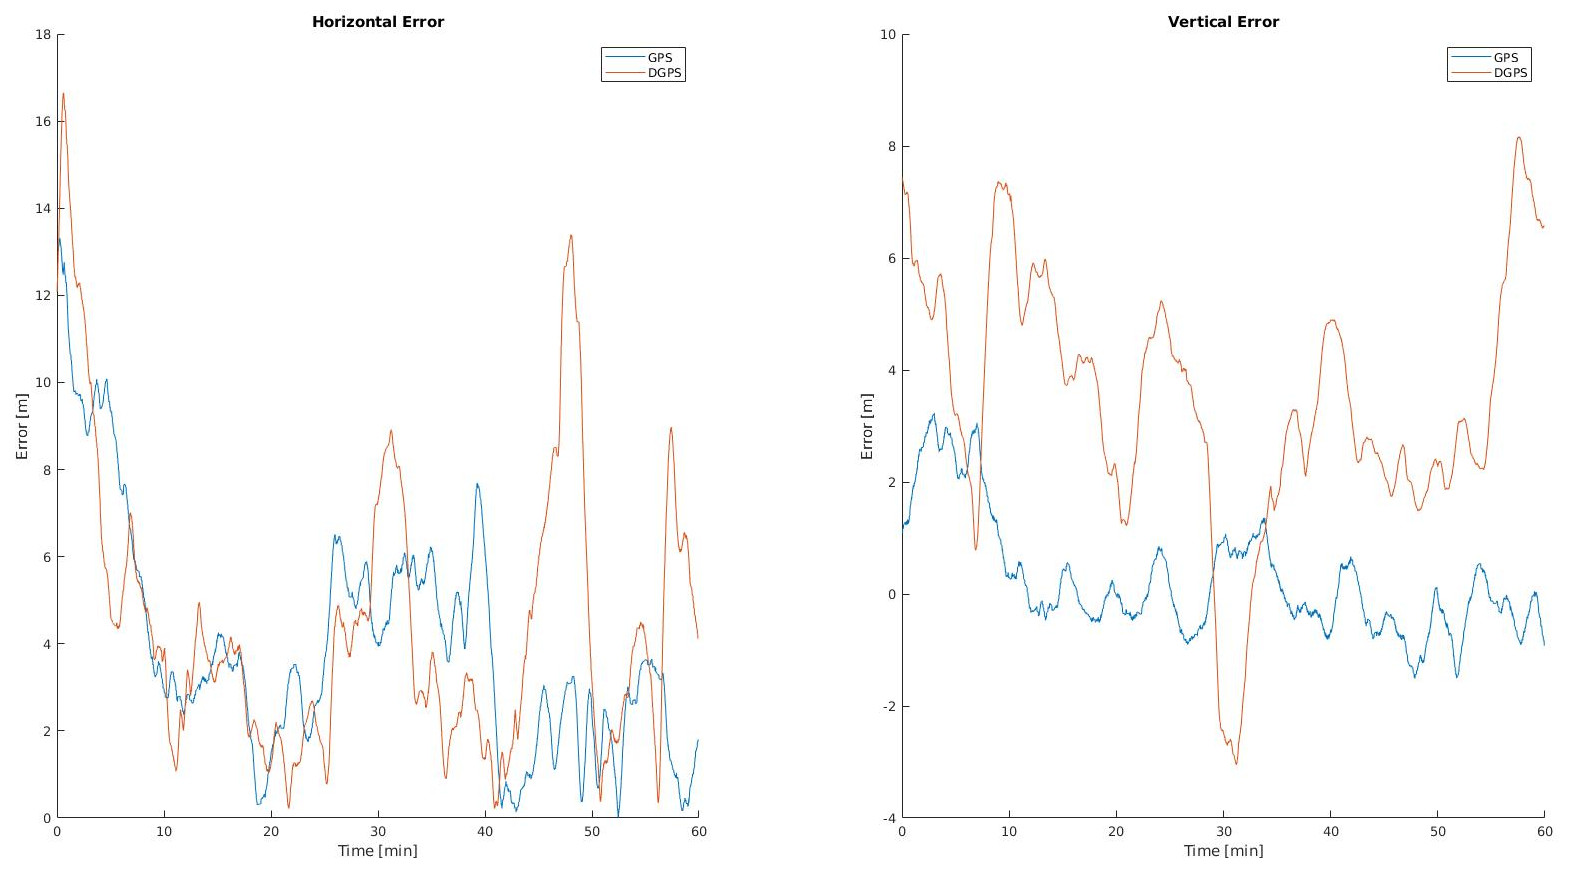
\includegraphics[width=\textwidth]{images/Errors_Kriens.jpg}
 \end{figure}
\end{frame}

\begin{frame}{Sonnenberg: Pseudorange Corrections}
 \begin{figure}
  \centering
  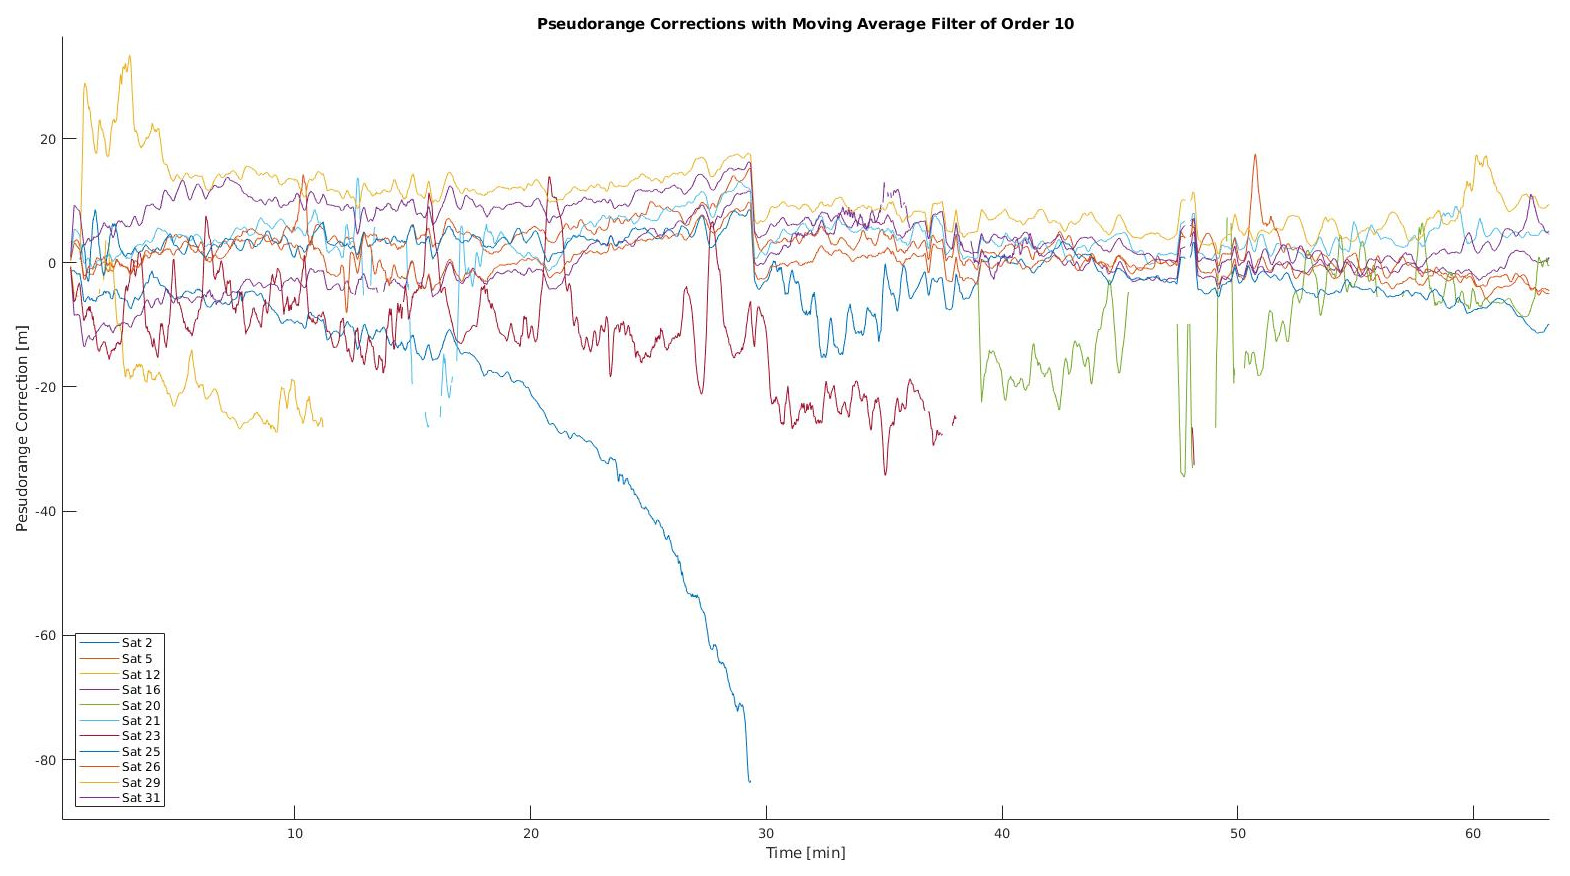
\includegraphics[width=\textwidth]{images/PRCs_Kriens.jpg}
 \end{figure}
\end{frame}


\section{Conclusion}

\begin{frame}{Conclusion}
 
\end{frame}


\begin{frame}[standout]
 Questions?
\end{frame}


\end{document}
